\documentclass{article}

\def\ParSkip{} 
\input{../../common/ryantibs}
\usepackage[normalem]{ulem}
\usepackage{animate}

\title{Calibration and Forecast Scoring \\ \smallskip
\large Advanced Topics in Statistical Learning, Spring 2023 \\ \smallskip
Ryan Tibshirani }
\date{}

\begin{document}
\maketitle
\RaggedRight
\vspace{-50pt}

\section{Introduction}

In this lecture, we cover a topic that sits adjacent to conformal prediction in
a sense, which is calibration. We will cover the perspective(s) on calibration 
from the forecasting literature, where it is arguably the most developed. 
Instead of focusing solely on calibration, we'll cover some of the broader
theory of forecasting, pertaining to scoring rules, calibration, and ensembles.     

There is a rich literature on forecast scoring and calibration. This literature
has roots in statistics, but over the years it has been expanded and driven by
applied forecasting disciplines, primarily weather forecasting. It is still
quite an active area in terms of development: new results that seem foundational
in nature are still being discovered year to year.  

As per our usual comment, what we cover in this lecture is only a sample of what
is known in the theory of forecasting. Unlike other topics, we are not aware of
a book that gives a modern and comprehensive treatment of forecast scoring
rules, calibration, and so on. (Perhaps this would be premature, as these topics
are still in active development, and such a book will come later.) One of the
most active and influential researchers in forecasting theory today is Tilmann
Gneiting, and much of what we cover will be drawing from his work with
collaborators, such as \citet{gneiting2007strictly, gneiting2007probabilistic,
    ranjan2010combining, gneiting2013combining}.

\subsection{Probabilistic forecasting}

Our setup in this lecture will be that of \emph{probabilistic} (as opposed to
\emph{point}) forecasting. In this setting, a forecaster outputs a predicted
distribution $P$ of a given target $Y$ of interest. We will generally focus on
the case in which $Y$ is real-valued.

In probabilistic forecasting, both $P$ and $Y$ are random variables. To help
give context, we can think of an underlying sequential problem indexed by time
$t=1,2,3,\dots$, where:
\[
\text{a forecaster predicts $P_t$ for the distribution of $Y_t$, based on
  information available at times $s<t$}.
\]
Sometimes it will be more convenient to make the time dependence explicit in the
notation, but often it will be more convenient to hide it. 

\subsection{Probabilities or quantiles?}

It is most common to represent a probabilistic forecast $P$ by its cumulative
distribution function (CDF) $F$. Of course, instead of representing $P$ by its
CDF $F$, we can choose to represent it by its quantile function $Q$. 
\emph{Typically these objects (CDF $F$ or quantile function $Q$) will be
  discretized in practice, and converting from one to the other will not be
  possible/practical, particularly in the tails}.Therefore, whether we choose at
the outset to represent a predicted distribution by a CDF or quantile function 
can have nontrivial implications on what tools we have at our disposal for
downstream tasks, like evaluation (via scoring rules) and aggregation.   

Later, in Section \ref{sec:prob_vs_quant}, we will discuss the differences
between aggregating probabilities (CDFs) and aggregating quantiles, in
detail. Here, we provide some higher-level practical considerations to keep in
mind when choosing to represent forecasts via probabilities versus quantiles.  

\begin{itemize}
\item A quantile representation for forecasts alleviates concerns about choosing
  the ``right'' bins for probability forecasts. Choosing bins in practice can be
  highly nonobvious, both in terms of the ``right''  scale, and the ``right''
  range.  

\item Quantiles can be directly fit a straightforward way, via quantile
  regression, and this can be carried out jointly over multiple probability
  levels. Constructing flexible (conditional) probability distributions can
  often be a more complex modeling task.  

\item For a discrete response that is concentrated around low values (such as 
  counts), a quantile representation may be undesirable since ``exact''
  quantiles only exist at a coarse set of probability levels (e.g., a reported
  level 0.05 quantile may actually be a level 0.09 quantile).     
\end{itemize}

\section{Scoring rules}

We now turn to discussing scoring rules, for evaluating probabilistic
forecasts. A \emph{scoring rule} (or simply a score) is a function $S$ that maps
a predicted distribution $P$ and target value $y$ to a real or infinite number 
\smash{$S(P, y) \in \widebar\R$} (where \smash{$\widebar\R = \R \cup \{\pm 
  \infty\}$} denotes the extended reals). We will, by convention, always take
the score to be negatively-oriented: a lower value means a better forecast.    

We use the notation $S(P, Q)$ to denote the expectation of the score over draws
$Y \sim Q$,  
\[
S(P, Q) = \E_{Y \sim Q} [S(P, Q)] = \int S(P, y) \, dQ(y).
\]

\subsection{Proper scores}

A scoring rule $S$ is said to be \emph{proper} if
\begin{equation}
\label{eq:proper}
S(P, Q) \geq S(Q, Q), \quad \text{for all $P,Q$},
\end{equation}
and \emph{strictly proper} if strict inequality holds in \eqref{eq:proper} for
$P \not= Q$. To quote \citet{gneiting2007strictly}, when $Q$ denotes the 
distribution of $Y$ and the score $S$ is proper: ``the forecaster has no
incentive to predict any $P \not= Q$ and is encouraged to report his or her true
belief''.  

Several examples of popular proper scores a given below. Some intuitively
appealing but improper scores are given as well. Throughout, we will write the 
scores as functions of densities, CDFs, quantile functions, etc.\ (instead 
of distributions), as convenient.  

\paragraph{Log score.}

\def\KL{\mathrm{KL}}

For a forecast that has density or probability mass function $p$, \emph{log
  score} is defined by 
\begin{equation}
\label{eq:logs}
\mathrm{LogS}(p, y) = -\log p(y).
\end{equation}
This is a strictly proper score. To see this, we compute:
\begin{equation}
\label{eq:kl_div}
\mathrm{LogS}(p, q) - \mathrm{LogS}(q, q) = \int \log \frac{q(y)}{p(y)} q(y) \, 
dy,
\end{equation}
which recall is the Kullback-Leibler (KL) divergence between $q$ and $p$, often
denoted $\KL(q,p)$ (note carefully the order of arguments here). This is known
to be nonnegative, and positive for $p \not= q$.

Log score \eqref{eq:logs} very sharply penalizes forecasts that place
insufficiently low probability on events that materialize: for small $p(y)$, the
score $-\log p(y)$ is very large (and asymptotes at $p(y) = 0$).  

\paragraph{Interlude: connection to Bergman divergence.}

KL divergence is a special instance of a \emph{Bregman divergence}, which is of
the form (note carefully the order of arguments)
\begin{equation}
\label{eq:bregman}
d_\phi(q,p) = \phi(q) - \phi(p) - \langle D\phi(p), q - p \rangle,
\end{equation}
for a convex differentiable function $\phi$, with derivative $D\phi$, and
suitable inner product $\langle \cdot, \cdot \rangle$. In particular, KL
divergence \eqref{eq:kl_div} is a Bregman divergence \eqref{eq:bregman} when
$\phi(p) = \int p(y) \log p(y) \, dy$, and $\langle p, q \rangle = \int p(y)
q(y) \, dy$.   

The connection between log score and Bregman divergence is no coincidence, and
the connection between proper scores and Bregman divergences runs much
deeper. If $\phi$ is strictly convex, then by the first-order characterization
for convexity, we have $d_\phi(q,p) \geq 0$, with strict inequality for $p \not= 
q$. Due to this fact, if $S$ is any score for which we have the Bregman
representation (for strictly convex $\phi$)   
\begin{equation}
\label{eq:bregman_rep}
S(p, q) - S(q, q) = d_\phi(q, p),
\end{equation}
then $S$ is strictly proper. In essence, the converse is true as well. The
formal details will be covered in Section \ref{sec:bregman_rep}. 

\paragraph{Quadratic score.}

For a forecast that has density or probability mass function $p$,
\emph{quadratic} or \emph{Brier score} is defined by   
\begin{equation}
\label{eq:quads}
\mathrm{QuadS}(p, y) = 2p(y) - \|p\|_2^2,
\end{equation}
where $\|p\|_2^2 = \int p(y)^2 \, dy$. This is a strictly proper score. To see
this, we compute:  
\[
S(p, q) - S(q, q) = \|p\|_2^2 - 2 \int p(y) q(y) \, dy + \|q\|_2^2 =
\|p-q\|_2^2,
\]
which is the $L^2$ distance between $p$ and $q$. Thus it is nonnegative, and
positive for $p \not= q$.  

Quadratic score \eqref{eq:quads} is more robust than log score \eqref{eq:logs},
in the sense that it is gentler in penalizing forecasts that place low
probability on events that materialize.  

\paragraph{Linear score.}

For a forecast that has density or probability mass function $p$,
\emph{linear score} is defined by   
\[
\mathrm{LinS}(p, y) = -p(y).
\]
We mention this score because it may seem intuitively appealing, but is
\emph{not proper} (and is basically never used in practice). To see this, let
$q$ be the standard normal density, and let $p$ be the uniform density on the 
interval $(-\epsilon, \epsilon)$, for some $\epsilon>0$ to be specified
later. Then    
\begin{align*}
\mathrm{LinS}(p, q) - \mathrm{LinS}(q, q) 
&= \int q(y)^2 \, dy - \frac{1}{2\epsilon} 
  \int_{-\epsilon}^\epsilon q(y) \, dy \\
&= \frac{1}{2\pi} \int e^{-y^2} \, dy -  \frac{1}{\sqrt{2\pi}}
  \frac{1}{2\epsilon} \int_{-\epsilon}^\epsilon e^{-y^2/2} \, dy \\   
&= \frac{1}{\sqrt{2\pi}} \bigg( 1/\sqrt{2} - \frac{1}{2\epsilon}
\int_{-\epsilon}^\epsilon e^{-y^2/2} \, dy \bigg).
\end{align*}
The last display will be negative for small enough $\epsilon > 0$: in 
particular, for \smash{$\epsilon < \sqrt{\log 2}$}, the integrand in the above
satisfies \smash{$e^{-y^2/2} > 1/\sqrt{2}$}, so the integral satisfies
\smash{$\frac{1}{2\epsilon}  \int_{-\epsilon}^\epsilon e^{-y^2/2} \, dy > 
  1/\sqrt{2}$}.

\paragraph{Continuous ranked probability score.}

Not all probabilistic forecasts can be expressed in terms of a density or
probability mass function. For example, some forecast distributions might place
a point mass at zero, and would be otherwise continuous. The \emph{continuous
  ranked probability score} (CRPS) accommodates this and, in general, any
forecast expressed in terms of a predicted CDF $F$. It is defined by 
\begin{equation}
\label{eq:crps}
\mathrm{CRPS}(F, y) = -\int (F(x) - 1\{y \leq x\})^2 \, dx. 
\end{equation}
This is a strictly proper score. To see this, we compute: 
\begin{align*}
\mathrm{CRPS}(F, G) - \mathrm{CRPS}(G ,G) 
&= \int \Big( G(x)^2 - F(x)^2 + 2(F(x) - G(x)) \E_{Y \sim G}[ 1\{Y \leq x\} ]
  \Big) \, dx \\
&= \int \Big( G(x)^2 - F(x)^2 + 2(F(x) - G(x)) G(x) \Big) \, dx \\
&= \int (F(x) - G(x))^2 \, dx.
\end{align*}
This is known as the Cram{\'e}r-von Mises distance between $F$ and $G$. Thus it
is nonnegative, and positive for $p \not= q$.  

CRPS \eqref{eq:crps} has become recently quite popular in various applied
forecasting communities (e.g., in meterological sciences), in part because it is
considered more robust than log score, and as already mentioned, it is more
broadly applicable, beyond log \eqref{eq:logs} and quadratic \eqref{eq:quads}
scores. However, unlike the latter two, CRPS is nontrivial to compute. Some
authors have pursued quadrature-based approximations to the integral defining
CRPS. A simpler approximation is given by noting its connection to weighted
interval score/quantile loss, which will be covered shortly.

\paragraph{Interval score.}

For an interval forecast expressed as $[\ell_\alpha, u_\alpha]$, where the lower
and upper endpoints $\ell_\alpha = Q(\alpha/2)$ and $u_\alpha = Q(1-\alpha/2)$
are the predicted $\alpha/2$ and $1-\alpha/2$ quantiles of the forecast
distribution $Q$, \emph{interval score} is defined by
\[
\mathrm{IS}_\alpha( [\ell_\alpha, u_\alpha], y) = 
(u_\alpha - \ell_\alpha) + \frac{2}{\alpha} \cdot
\mathrm{dist}(y, [\ell_\alpha, u_\alpha])
\]
where \smash{$\mathrm{dist}(y, S) = \inf_{x \in S} |x-y|$} for a set $S$. We can
see that this combines a reward for sharpness (first term) and a penalty for 
miscoverage (second term). For a collection of interval forecasts
$[\ell_\alpha, u_\alpha]$, $\alpha \in \cA$, \emph{weighted interval score}
(WIS) is defined by
\begin{align}
\nonumber
\mathrm{WIS}_\cA \big( \{[\ell_\alpha, u_\alpha]\}_{\alpha \in \cA}, \, y \big)  
&= \sum_{\alpha \in \cA} \alpha \cdot \mathrm{IS}_\alpha( [\ell_\alpha,
  u_\alpha], y) \\
\label{eq:wis}
&=\sum_{\alpha \in \cA} \Big(\alpha (u_\alpha - \ell_\alpha) + 2 \cdot
  \mathrm{dist}(Y, [\ell_\alpha, u_\alpha]) \Big).
\end{align}
Weighted interval score (and thus interval score, as effectively a special case)
is a proper score for predicting the quantiles at levels $\alpha/2$ and
$1-\alpha/2$, over $\alpha \in \cA$. To be clear, here we say (by analogy to 
\eqref{eq:proper}) that a score $S$ defined in terms of a discrete set of
predicted quantiles \smash{$\{q_\tau\}_{\tau \in \cT}$} is proper if (for $Q$
denoting the true quantile function of the distribution of $Y$) it holds that   
\begin{equation}
\label{eq:proper_q}
S \big( \{q_\tau\}_{\tau \in \cT}, \, Q \big) \geq S \big( \{Q(\tau)\}_{\tau \in
  \cT}, \, Q \big), \quad \text{for all $\{q_\tau\}_{\tau \in \cT}$, and all
  $Q$},   
\end{equation}
where as usual \smash{$S(\{q_\tau\}_{\tau \in \cT}, \, Q) = \E_{Y \sim Q}[
  S(\{q_\tau\}_{\tau \in \cT}, \, Q)]$}. Propriety of weighted interval score
can be verified by drawing a connection to quantile loss, covered next. 

\paragraph{Quantile score.}

For a forecast expressed as a collection of predicted quantiles $q_\tau$, $\tau
\in \cT$, \emph{quantile score} (QS) is defined by 
\begin{equation}
\label{eq:qs}
\mathrm{QS}_\cT \big( \{q_\tau\}_{\tau \in \cT}, \, y \big) = 
\sum_{\tau \in \cT} \rho_\tau(y - q_\tau),
\end{equation}
where $\rho_\tau(u) = \tau |u|$ for $u \geq 0$ and $(1-\tau) |u|$ for $u < 0$,
often called the tilted $\ell_1$ loss at the level $\tau$. This is nothing else
than the loss that is the standard choice in \emph{quantile regression}. That
quantile score is proper, in the sense of \eqref{eq:proper_q}, follows from the
standard fact that the true level $\tau$ quantile is a minimizer of the expected
tilted $\ell_1$ loss at the level $\tau$.

\paragraph{Connection between WIS and QS.}

The following is an connection between WIS \eqref{eq:wis} and QS \eqref{eq:qs}: 
for any set $\cA$ of error levels, if we define a corresponding set
\smash{$\cT = \cup_{\alpha \in \cT} \, \{ \alpha/2, 1-\alpha/2 \}$} of
probability levels, then it holds that     
\begin{equation}
\label{eq:wis_qs}
\mathrm{WIS}_\cA \big( \{[\ell_\alpha, u_\alpha]\}_{\alpha \in \cA}, \, y \big)  
= 2 \cdot \mathrm{QS}_\cT \big( \{q_\tau\}_{\tau \in \cT}, \, y \big).
\end{equation}
The equivalence \eqref{eq:wis_qs} between WIS and QS can be verified by
straightforward algebra. Apart from being interesting, and lending a new 
interpretation to how quantile score \eqref{eq:qs} combines a sharpness reward
with a miscoverage penalty (recall the discussion following \eqref{eq:wis}), it
is also a useful observation as it provides an indirect but simple proof that
WIS \eqref{eq:wis} is proper, in the sense of \eqref{eq:proper_q}.

\paragraph{Connection between CRPS and QS.}

The connections continue: interestingly, CRPS \eqref{eq:crps} also has an
equivalent formulation in terms of QS: if $F$ differentiable, with density $f$,
and admits an expectation, $\int y f(x) \, dy < \infty$, then    
\begin{equation}
\label{eq:crps_qs}
\int (F(x) - 1\{y \leq x\})^2 \, dx = 
2 \int \rho_\tau(y - F^{-1}(\tau)) \, d\tau. 
\end{equation}
The right-hand side is an integral of QS all probability levels $\tau \in [0,1]$.
This is quite interesting because these two error metrics---CRPS and QS---are 
motivated from very different perspectives, not to mention different
parametrizations (CDF space versus quantile space).   

The equivalence in \eqref{eq:crps_qs} appears to have been discovered by
\citet{laio2007verification}; their argument uses integration by parts, but it
ignores a few subtleties, and hence below we reproduce the proof from
\citet{fakoor2021flexible}, which basically just fills in a few missing details.   
Starting with the right-hand side in \eqref{eq:crps_qs}, we can substitute
$y=F^{-1}(\tau)$ to rewrite the integral as   
\[
2 \int (1\{y \leq F^{-1}(\tau)\} - \tau) (F^{-1}(\tau)-X) \, d\tau =  
2 \int (1\{y \leq x\} - F(x)) (x-y) f(x) \, dx.
\]
Let $u'(x)=2(1\{y \leq x\} - F(x)) f(x)$ and $v(x)=x-y$. The idea is now to use 
integration by parts, but there are two subtleties. First, one has to be careful 
about framing the antiderivative $u$ of $u'$, since $x \mapsto 1\{y \leq x\}$ is
not classically differentiable. Note that we can actually redefine $u'$ to be   
\[
u'(x) = 2(1\{y \leq x\} - F(x)) (f(x) - \delta_y(x)),
\]
where $\delta_y$ is the Dirac delta function centered at $y$, because the
``extra'' piece integrates to zero:   
\[
\int 2(1\{y \leq x\} - F(x)) (x-y) \delta_y(x) \, dx =  
2(1\{y \leq x\} - F(x)) (x-y) \Big|_{x=y} = 0. 
\]
With this new definition of $u'$, its antiderivative is rigorously
\[
u(x) = -(1\{y \leq x\} - F(x))^2,
\] 
because, in the distributional sense, the derivative of the heavyside function
$x \mapsto 1\{y \leq x\}$ is indeed the delta function $\delta_y$. Thus we have   
\begin{align*}
\int u'(x) v(x) \, dx
&= u(x) v(x) \Big|_{-\infty}^\infty - \int u(x) v'(x) \,  dx \\ 
&= -(1\{y \leq x\} - F(x))^2 (x-y) \Big|_{-\infty}^\infty + 
\int (1\{y \leq x\} - F(x))^2 \, dx. 
\end{align*}
The second subtlety is to show that the first term above is indeed zero.  
This is really a question of how fast the tails of $F$ decay. As $F$ yields an
expectation, note that we must have $1-F(x) \lesssim x^{-p}$ for $p>1$ (since
$1/x$ is not integrable on any one-sided interval $[q,\infty)$ for $q>0$). Hence   
\[
(1-F(x)) x \lesssim x^{-p+1} \to 1 \quad \text{as $x \to \infty$},
\]
and the other limit, as $x \to -\infty$, is similar.

\paragraph{Quick recap.}

Here is a quick recap of what we learned on our tour of scores. Log score
\eqref{eq:logs} and quadratic score \eqref{eq:quads} are classical choices, each
strictly proper, with the former being more aggressive at penalizing
underconfidence assigned to rare events. CRPS \eqref{eq:crps} is a more modern
alternative, also strictly proper, which has become popular due to its
robustness and generality (it applies to any CDF). However, it is nontrivial to
compute.     

For forecasts specified in terms of quantiles at discrete probability levels,
WIS \eqref{eq:wis} and QS \eqref{eq:qs} are each proper, simple, and popular
choices, motivated from different perspectives; and in fact they turn out to be 
equivalent \eqref{eq:wis_qs}. Moreover, CRPS turns out to be equivalent
to an integrated quantile score \eqref{eq:crps_qs} over all probability
levels. Thus a simple approximation to CRPS in practice would be to discretize
at any desired set of probability levels and use this to define WIS/QS;
propriety is always maintained, in the sense of \eqref{eq:proper_q}, for any
choice of discretization.     

Figures \ref{fig:scores1} and \ref{fig:scores2} visualize the various scores in
action. 

\begin{figure}[p]
\centering
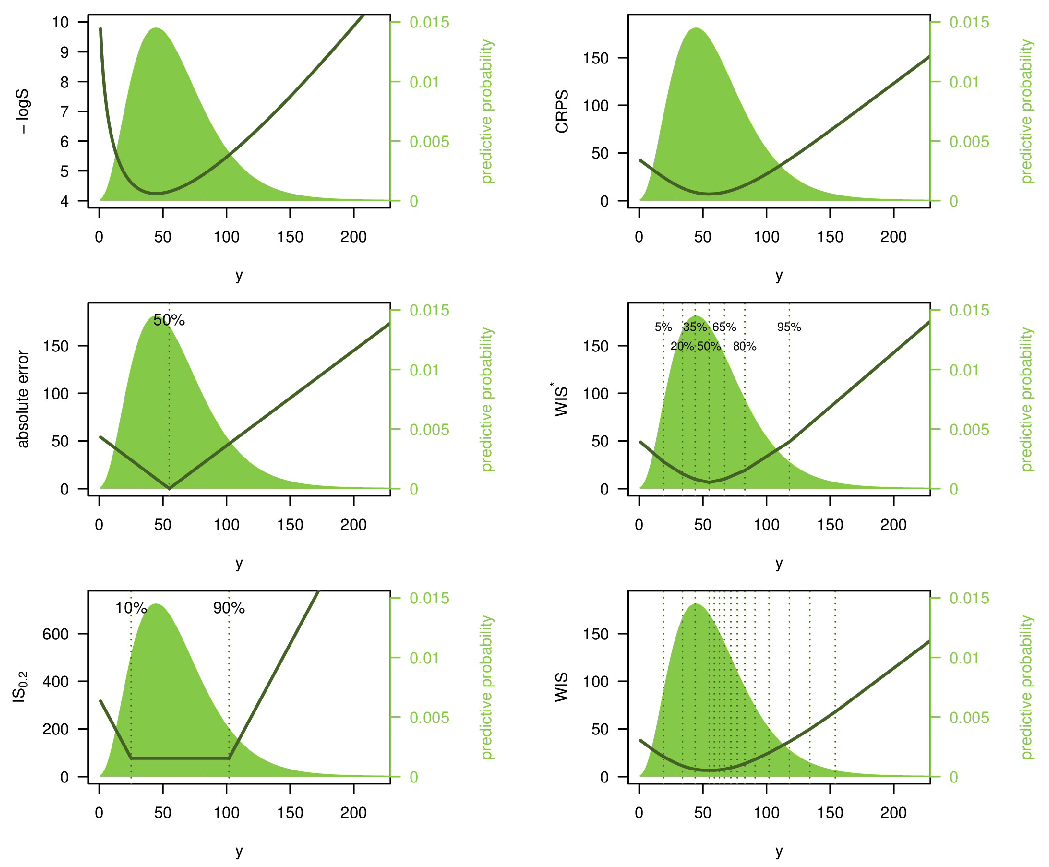
\includegraphics[width=0.975\textwidth]{scores1.png}
\caption{\it Various scores visualized as functions of $y$, based on the
  predicted distribution plotted in green. Here WIS$^*$ and WIS denote two
  versions of weighted interval score at a coarser and finer set of probability
  levels, respectively. Credit: \citet{bracher2021evaluating}.}       
\label{fig:scores1}   

\bigskip\medskip

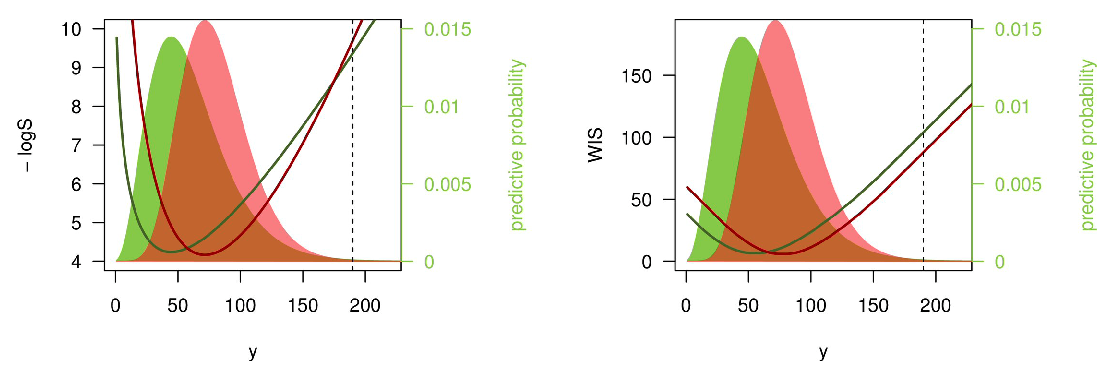
\includegraphics[width=0.975\textwidth]{scores2.png}
\caption{\it Comparison between log score and WIS for two predicted
  distributions, $P$ in green and $Q$ in red. We see that $G$ has higher
  expectation, while $F$ is more dispersed. The event $y$ that materializes is
  visualized as a dashed vertical line. Log score prefers $F$ to $G$, while WIS
  prefers $G$ to $F$. Credit: \citet{bracher2021evaluating}.}          
\label{fig:scores2}
\end{figure}

\subsection{Bregman representation}
\label{sec:bregman_rep}

Below we state an important result from \citet{gneiting2007strictly} that shows
that the Bregman representation \eqref{eq:bregman_rep} which we saw was possible 
for log score (and quadratic score, and CRPS) is ``no accident'', and in a
precise sense, characterizes \emph{all} proper scores.    

Before stating the result, we must introduce some terminology and
concepts. Recall that by convention, we take all scores to be
negatively-oriented. First, we say a score $S$ is \emph{regular} if $S(P,P)$ is 
real-valued for all $P$ (i.e., we allow $S(P,Q) = \infty$ for $P \not=
Q$). Regularity is essentially needed in order for subderivatives (defined 
shortly) to make sense but we omit the details. 

Next, we refine the definition of propriety: for a class $\cP$ of probability
distributions, we say a score $S$ is \emph{proper relative to $\cP$} if
\eqref{eq:proper} holds for $P,Q \in \cP$, with \emph{strictly proper relative 
  to $\cP$} again meaning that the inequality is strict for $P \not= Q$.  

Lastly, for a function $\phi$ acting over a set of distributions $\cP$, with
each $P \in \cP$ having a sample space $\cY$, we say that $D\phi(P, \cdot)$ is a
\emph{subderivative} of $\phi$ at $P \in \cP$ provided that 
\begin{equation}
\label{eq:subderiv}
\phi(Q) \geq \phi(P) + \int D\phi(P, y) \, d(Q-P)(y), \quad \text{for all $Q \in
  \cP$}.  
\end{equation}

We are now ready to state the result. 

\begin{theorem}
Let $\phi$ be convex function acting over a set of distributions $\cP$. Define
for $P \in \cP$ and $y \in \cY$ the regular score  
\begin{equation}
\label{eq:phi_score}
S(P, y) = -\phi(P) - D\phi(P, y) + \int D\phi(P, y) \, dP(y),
\end{equation}
where $D\phi(P, \cdot)$ is a subderivative of $\phi$ at $P$. Then for any $P,Q
\in \cP$, 
\begin{equation}
\label{eq:phi_div}
S(P, Q) - S(Q, Q) = \underbrace{\phi(Q) - \phi(P) - \int D\phi(P, y) \,
  d(Q-P)(y)}_{d_\phi(Q,P)},
\end{equation}
which is the Bregman divergence with respect to $\phi$, and the score $S$ is
proper relative to $\cP$.  

Conversely, if $S$ is a regular score that is proper relative to $\cP$, then $S$
can be written in the form \eqref{eq:phi_score} with respect to the convex
function $\phi(P) = -S(P, P)$, and the Bregman representation \eqref{eq:phi_div}
holds.    

Finally, the above equivalence also holds when the terms convex and proper are
replaced by strictly convex and strictly proper, respectively.  
\end{theorem}

\begin{proof}
If $\phi$ is convex and we define $S$ according to \eqref{eq:phi_score}, then
\eqref{eq:phi_div} follows by direct algebra. Meanwhile, $d_\phi(Q, P) \geq 0$
for any $P,Q \in \cP$ by definition of the subderivative \eqref{eq:subderiv},
which proves that $S$ is proper relative to $\cP$. For the other direction, if
$S$ is regular and proper relative to $\cP$, then letting $\phi(Q) = -S(Q, Q)$
is equivalent to letting  
\[
\phi(Q) = -\inf_{P \in \cP} \, S(P, Q) = \sup_{P \in \cP} \, -S(P, Q).
\]
For fixed $P$, the function $Q \mapsto -S(P, Q)$ is linear, and hence convex,
and thus by the above $\phi$ is a pointwise supremum of convex functions and
hence itself convex. Furthermore, we can see that $D\phi(P, \cdot) = -S(P,
\cdot)$ is a valid subderivative of $\phi$, since \eqref{eq:subderiv} becomes 
$-S(Q,Q) \geq -S(P,Q)$ for all $Q \in \cP$, which is satisfied because $S$ is
proper relative to $\cP$. Under the choice $D\phi(P, \cdot) = -S(P, \cdot)$, the 
score representation \eqref{eq:phi_score} is a tautology, and again, the Bregman
representation \eqref{eq:phi_div} follows by direct algebra.

The arguments for strict convexity and strict propriety follow similarly.
\end{proof}

Even though our focus has been (and will continue to be) real-valued forecasts,
it is worth emphasizing that the previous theorem treats the sample space $\cY$
as arbitrary. In the case of categorical forecasts, where $\cY = \{1,\dots,k\}$,
we get the following corollary (which is originally due to 
\citet{savage1971elicitation}). We denote the standard $k$-dimensional
probability simplex by \smash{$\Delta^k = \{ p \in \R^k : p \geq 0, \;
  \sum_{i=1}^k p_i = 1\}$}.

\begin{corollary}
Let $\cY = \{1,\dots,k\}$. Then a regular score $S$, which we treat as acting on
a vector of probabilities $p \in \Delta^k$, is proper with respect to the set of
all distributions on $\{1,\dots,k\}$ if and only if 
\[
S(p, i) = -\phi(p) - D_i\phi(p) + \langle D\phi(p), p \rangle , \quad \text{for
  $i=1,\dots,k$},
\]
for a convex function $\phi$ on $\Delta^k$, where $D\phi(p)$ denotes the
subgradient of $\phi$ at $p$ (with components $D_i\phi(p)$, $i=1,\dots,k$). The
same equivalence also holds when the terms convex and proper are replaced by
strictly convex and strictly proper, respectively.     
\end{corollary}

\section{Modes of calibration}

\subsection{Probabilistic calibration}

\subsection{Marginal calibration}

\subsection{Conditional calibration}


\section{Aggregation and (mis)calibration}

\section{Probability versus quantile aggregation}
\label{sec:prob_vs_quant}

\bibliographystyle{plainnat}
\bibliography{../../common/ryantibs}

\end{document}
